\documentclass[../Article_Model_Parameters.tex]{subfiles}
\graphicspath{{\subfix{../Figures/}}}
\begin{document}
	
	\section{Materials and methods} \label{CH: Materials and methods}
	
	\subsection{Governing equations} \label{CH:Governing_equations_chapter}
	Following the work of \citet{Anderson1995}, the governing equations for quasi-one-dimensional were derived. Quasi-one-dimensional flow refers to a fluid flow scenario assuming that flow properties are uniformly distributed across any cross-section. This simplification is typically applied when the flow channel's cross-sectional area changes, such as through irregular shapes or partial fillings of an extractor. According to this assumption, velocity and other flow properties change solely in the flow direction.
	
	As discussed by \citet{Anderson2023}, all flows are compressible, but some of them can be treated as incompressible when the Mach number is smaller than 0.3. This assumption leads to the incompressible condition: $\nabla \cdot u =0$, which is valid for constant density (strict incompressible) or varying density flow. The assumption allows for removing acoustic waves and large perturbations in density and/or temperature. In the 1-D case, the incompressibility condition becomes $\frac{du}{dz} = 0$, so the fluid velocity is constant.
	
	The set of quasi-one-dimensional governing equations in Cartesian coordinates is described by Equations \ref{EQ: CompressibleEuler_1} - \ref{EQ: CompressibleEuler_3}.
	
	{\footnotesize
		\begin{align}
			\label{EQ: CompressibleEuler_1}
			\cfrac{\partial \left( \rho_f A_f \right) }{\partial t} + \cfrac{\partial \left( \rho_f A_f v \right)}{\partial z} &= 0 \\
			\cfrac{\partial \left( \rho_f v A_f \right) }{\partial t} + \cfrac{\partial \left( \rho_f A_f v^2 \right)}{\partial z} &= -A_f \cfrac{\partial P}{\partial z} \label{EQ: CompressibleEuler_2} \\
			\cfrac{\partial \left( \rho_f e A_f \right) }{\partial t} + \cfrac{\partial \left( \rho_f A_f v e\right)}{\partial z} &= -P\cfrac{\left( A_f v \right)}{\partial z} + \cfrac{\partial}{\partial z} \left( k \cfrac{\partial T}{\partial z} \right)   
			\label{EQ: CompressibleEuler_3}
		\end{align}  
	}
	
	where $\rho_f$ is the density of the fluid, $A_f$ is the function which describe change of the cross-section, $v$ is the velocity, $P$ is the total pressure, $e$ is the internal energy of the fluid, $t$ is time and $z$ is the spacial direction.
	
	\subsection{Extraction model} \label{CH: Extraction_model}
	\subsubsection{Continuity equation} \label{CH: Continuity}
	
	The previously derived quasi-one-dimensional continuity equation (Equation \ref{EQ: CompressibleEuler_1}) is redefined by incorporating a function $A_f = A\phi$. This modification distinguishes constant and varying terms, where the varying term accounts for the changes in the cross-sectional area available for the fluid. Equation \ref{EQ: Continuity_differential} shows the modified continuity equation:
	
	{\footnotesize
		\begin{equation} \label{EQ: Continuity_differential}
			\frac{\partial (\rho_f \phi)}{\partial t} + \frac{\partial (\rho_f v A\phi)}{\partial z} = 0
		\end{equation}
	}
	where $A$ is the total cross-section of the extractor and $\phi$ describes porosity along the extractor.
	
	Assuming that the mass flow rate is constant in time, the temporal derivative becomes the mass flux F, and the spatial derivative can be integrated along $z$ as
	
	{\footnotesize
		\begin{equation}
			\int \frac{\partial (\rho_f v A \phi )}{\partial z} dz = F \rightarrow F=\rho_f v A\phi
		\end{equation}
	}
	
	To simplify the system's dynamics, it is assumed that $F$ is a control variable and affects the whole system instantaneously (due to $\nabla \cdot u = 0$), which allows finding the velocity profile that satisfies mass continuity based on $F$, $\phi$, and $\rho_f$.
	
	{\footnotesize
		\begin{equation} \label{EQ:Velocity_1}
			v = \cfrac{F}{\rho_f A\phi} 
		\end{equation}
	}
	
	Similarly, the superficial velocity might be introduced.
	
	{\footnotesize
		\begin{equation} \label{EQ:Velocity_2}
			u = v \phi = \cfrac{F}{\rho_f A }
		\end{equation}
	}
	
	The fluid density $\rho_f$ can be obtained from an equation of state ({\color{red}article 1}) if temperature and thermodynamic pressure are known along $z$. The fluid density variation may occur due to pressure or inlet temperature changes. In the non-isothermal case, $\rho_f$ in Equations \ref{EQ:Velocity_1} and \ref{EQ:Velocity_2} is considered an average fluid density along the extraction column.
	
	\subsubsection{Mass balance for the fluid phase} \label{CH: Mass_balance_fluid}
	
	Equation \ref{Model_fluid} describes the movement of the solute in the system, which is constrained to the axial direction due to the quasi-one-dimensional assumption. Given that the solute concentration in the solvent is negligible, the fluid phase is described as pseudo-homogeneous, with properties identical to the solvent itself. It is also assumed that the thermodynamic pressure remains constant throughout the device. The analysis further simplifies the flow dynamics by disregarding the boundary layer near the extractor's inner wall. This leads to a uniform velocity profile across any cross-section perpendicular to the axial direction. Thus, the mass balance equation includes convection, diffusion, and kinetic terms representing the fluid phase behaviour.
	
	{\footnotesize
		\begin{equation}
			\label{Model_fluid}
			\frac{\partial c_f}{\partial t}
			+ \frac{1}{\phi} \frac{\partial \left( c_f u\right)}{\partial z}
			= \frac{1-\phi}{\phi} r_e
			+ \frac{1}{\phi} \frac{\partial}{\partial z} \left( D^M_e \frac{\partial c_f}{\partial z} \right)
		\end{equation}
	}
	
	$c_f$ represents the solute's concentration in the fluid phase, $r_e$ is a mass transfer kinetic term, and $D^M_e$ is the axial diffusion coefficient.
	
	\subsubsection{Mass balance for the solid phase} \label{Mass_balance_solid}
	
	As given by Equation \ref{Model_solid}, the solid phase is considered stationary, without convection and diffusion terms in the mass balance equation. Therefore, the only significant term in this equation is the kinetic term of Equation \ref{Model_kinetic_basic}, which connects the solid and fluid phases. For simplicity, the extract is represented by a single pseudo-component. 
	
	{\footnotesize
		\begin{equation} 
			\label{Model_solid}
			%		{\scriptsize\begin{equation}
					\cfrac{\partial c_s}{\partial t} = \underbrace{ r_e }_{\text{Kinetics}}
			\end{equation} }
			
			\subsubsection{Kinetic term} \label{CH: Kinetic}
			
			As the solvent flows through the bed, CO$_2$ molecules diffuse into the pores and adsorb on the particle surface to form an external fluid film around the solid particles due to the solvent-solid matrix interactions. The dissolved solute diffuses from the particle's core through the solid-fluid interface, the pore, and the film into the bulk. Figure \ref{fig: SFE_Mechanism} shows the mass transfer mechanism, where the mean solute concentration in the solid phase is denoted as $c_s$, and the equilibrium concentrations at the solid-fluid interface are denoted as $c_s^*$ and $c_p^*$, respectively, for solid and fluid phases. The concentration of the solutes in the fluid phase in the centre of the pore is denoted as $c_p$. As the solute diffuses through the pore, its concentration changes and reaches $c_{pf}$ at the pore's opening. Then, the solute diffuses through the film around the particle and reaches bulk concentration $c_f$. The two-film theory describes the solid-fluid interface inside the pore. The overall mass transfer coefficient can be determined from the relationship between the solute concentration in one phase and its equilibrium concentration.
			
			\begin{figure}[h!]
				\centering
				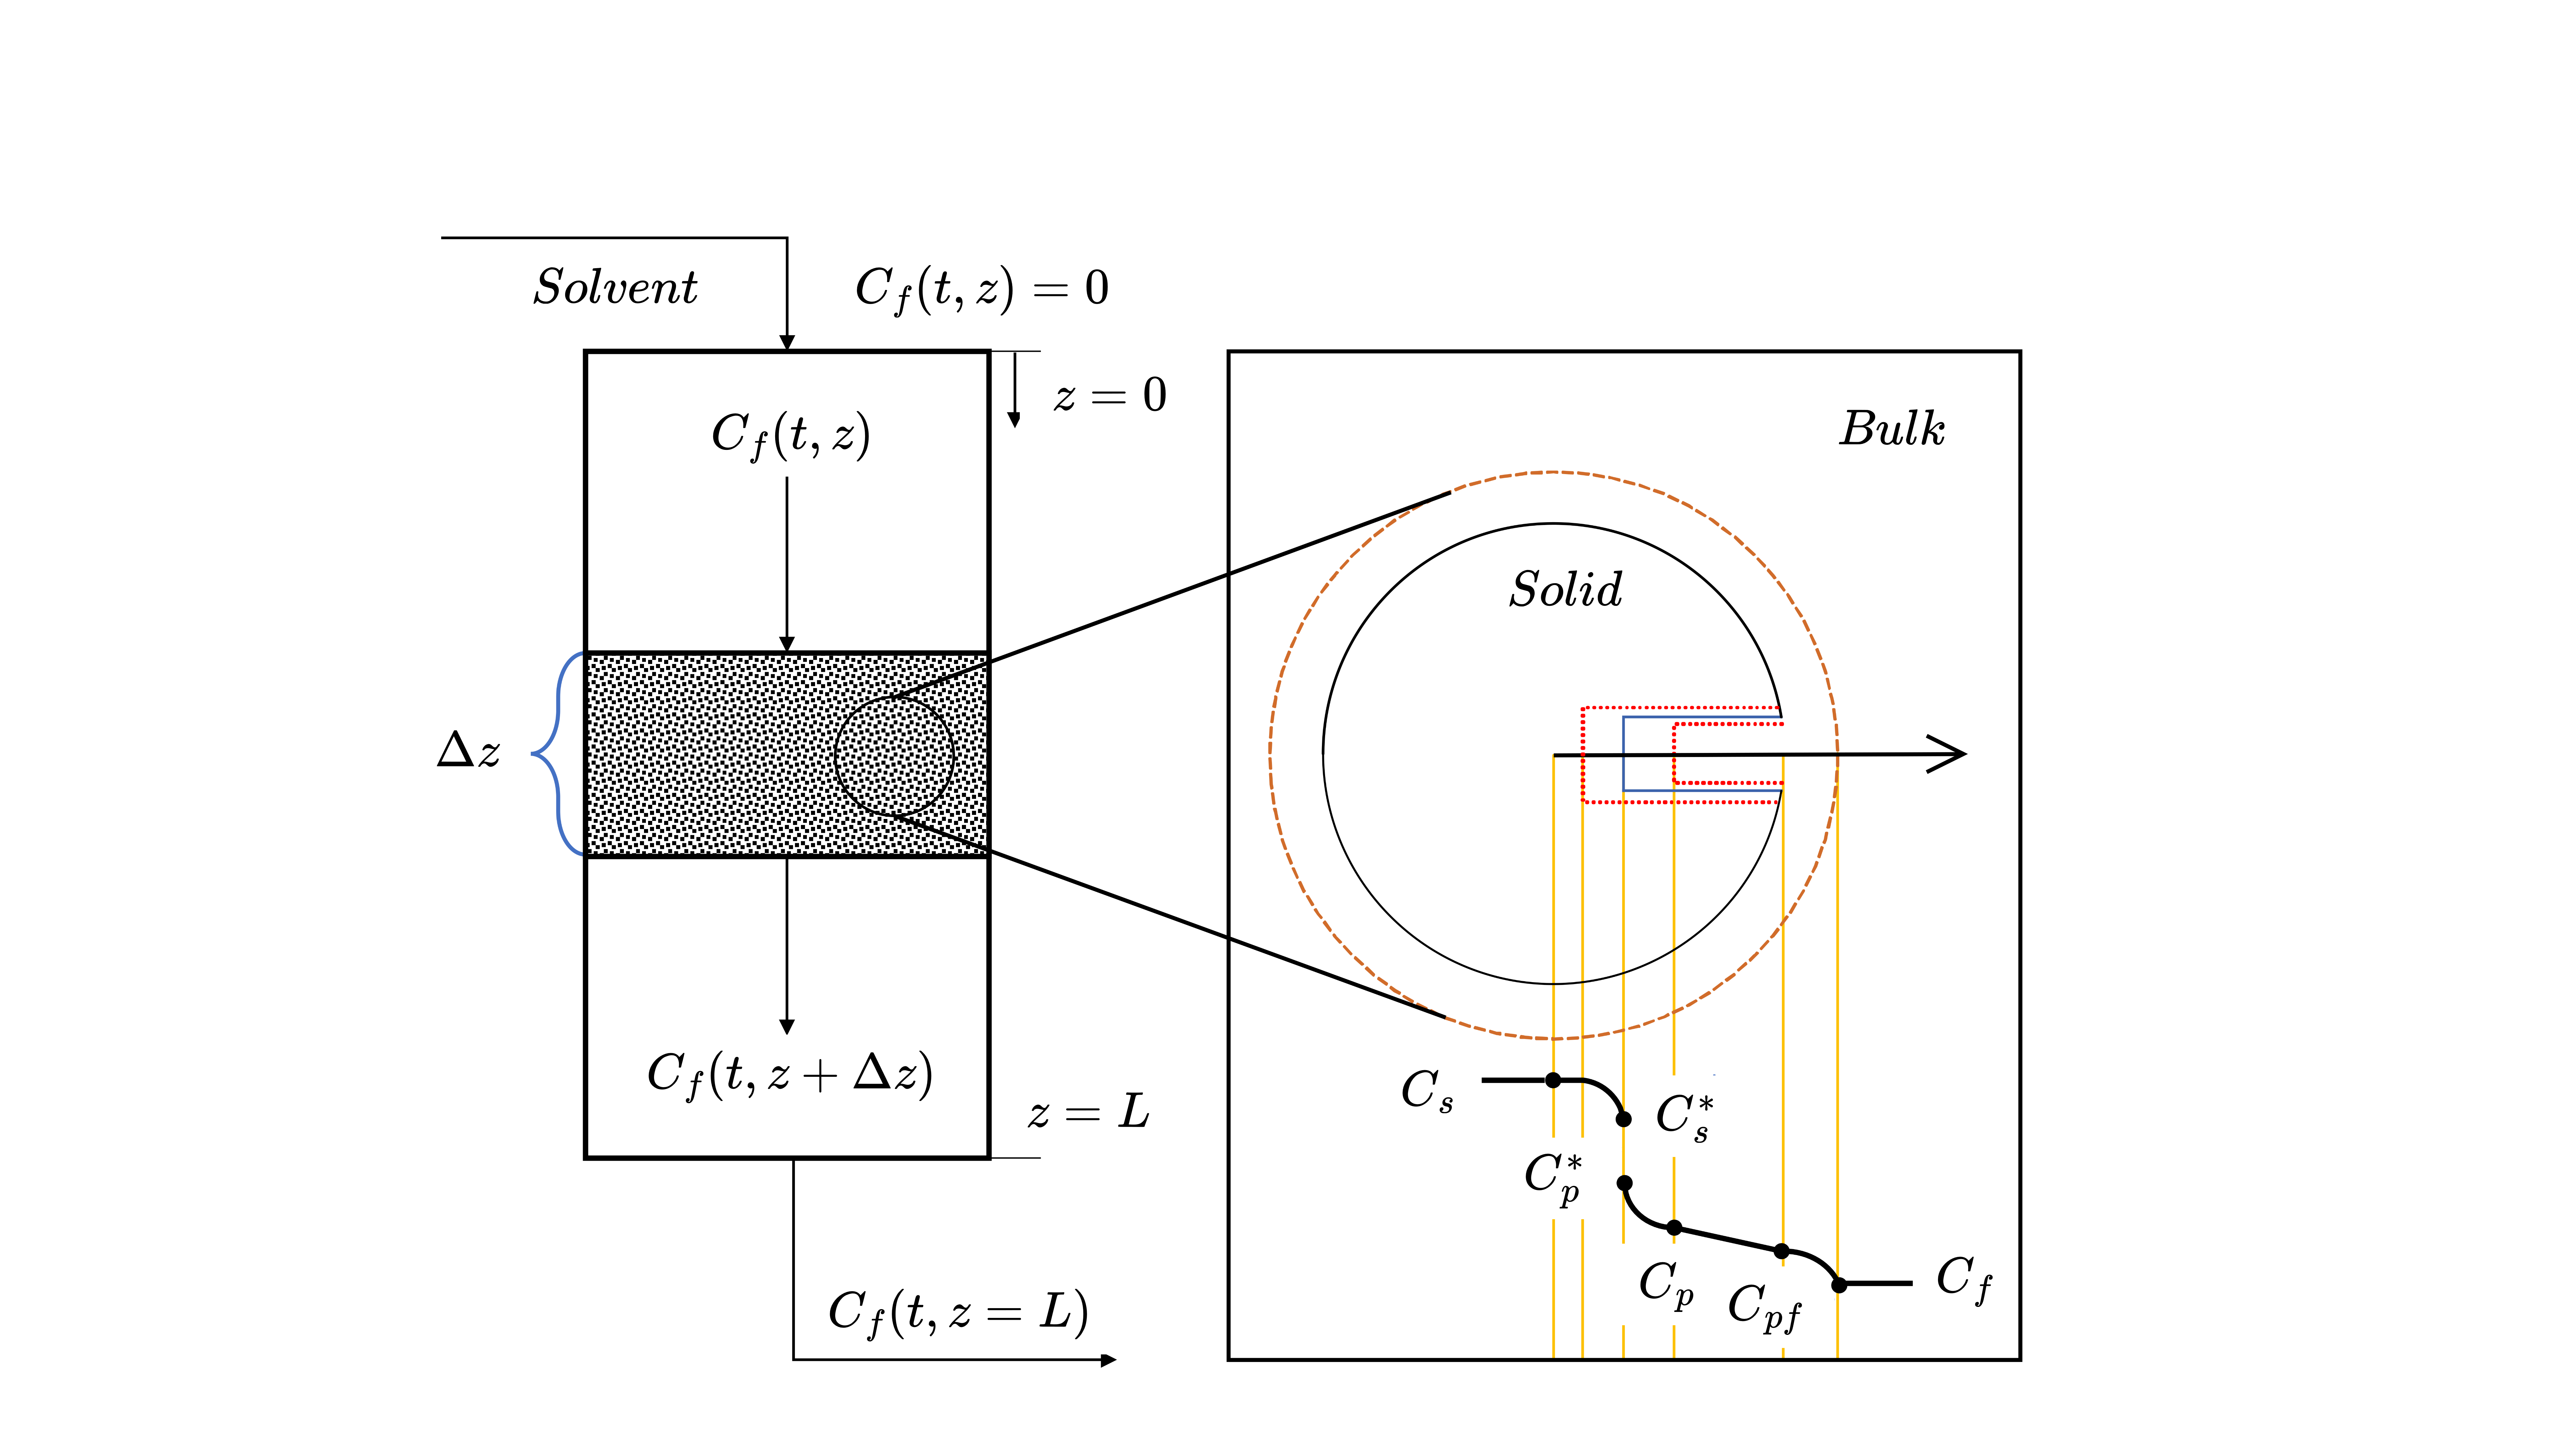
\includegraphics[trim = 45cm 0cm 60cm 20cm,clip,width=0.85\columnwidth]{Figures/SFE_PFD.drawio.png}	
				\caption{The mass transfer mechanism}
				\label{fig: SFE_Mechanism}
			\end{figure}
			
			\citet{Bulley1984} suggests a process where the driving force for extraction is given by the difference between the concentration of the solute in bulk, $c_f$, and in the centre of the pore, $c_p^*$. The concentration $c_p^*$ is in equilibrium with $c_s$ according to an equilibrium relationship. The rate of extraction is thus $r_e\left(c_f - c^*_p(c_s)\right)$. On the other hand, \citet{Reverchon1996} proposes a driving force given by the difference between $c_s$ and $c_p^*$. Concentration $c_p^*$ is determined by an equilibrium relationship with $c_f$ and the extraction rate given by Equation \ref{Model_kinetic_basic}
			
			{\footnotesize
				\begin{equation} \label{Model_kinetic_basic}
					r_e = \cfrac{D_i}{\mu l^2 }\left(c_s - c_p^* \right)
			\end{equation} }
			
			where $\mu$ is sphericity, $l$ a characteristic dimension of particles and can be defined as $l = r/3$, $r$ is the mean particle radius, $\rho_s$ is the solid density, $D_i$ corresponds to the overall diffusion coefficient and $c_P^*$ is a concentration at the solid-fluid interface (which according to the internal resistance model is supposed to be at equilibrium with the fluid phase). 
			
			According to \citet{Bulley1984}, a linear equilibrium relationship (Equation \ref{Linear_equilibirum}) can be used to find an equilibrium concentration of the solute in the fluid phase $c_f^*$ based on the concentration of the solute in the solid phase $c_s$.
			
			{\footnotesize
				\begin{align} \label{Linear_equilibirum}
					c_f^* &= k_p c_s
			\end{align} }
			
			The volumetric partition coefficient $k_p$ acts as an equilibrium constant between the solute concentration in one phase and the corresponding equilibrium concentration at the solid-fluid interphase. According to \citet{Spiro2007}, $k_p$ can be expressed through the mass partition coefficient $k_m$.
			
			{\footnotesize
				\begin{align}
					k_m = \cfrac{k_p \rho_s}{\rho_f}
			\end{align} }
			
			According to \citet{Reverchon1996}, the kinetic term becomes
			
			{\footnotesize
				\begin{equation}
					\label{Model_kinetic_no_sat}
					r_e = -\cfrac{D_i}{ \mu l^2 } \left(c_s - \cfrac{\rho_s c_f}{k_m \rho_f} \right)
			\end{equation} }
			
			\subfile{Saturation}
		
			\subsubsection{Pressure term} \label{CH: Pressure}
			
			The pressure term in the energy equation, given by Equation \ref{EQ:Enthalpy_equation}, describes the change of the thermodynamic pressure with respect to time. As explained in Chapters \ref{CH:Governing_equations_chapter}, at Low-Mach number conditions, the thermodynamic pressure is nearly constant in space due to the small pressure wave propagation that occurs at the speed of sound. Under such conditions, the term $\partial P/\partial t$ can be approximated by an difference equation, which describes the change of pressure in the whole system. The pressure ($P$) in the system is considered a state variable, while the pressure in the new time-step ($P_{in}$) is considered a control variable.
			
			{\footnotesize
				\begin{equation}
					\frac{\partial {\color{black}P}(t)}{\partial t} \approx \frac{{\color{black}P_{in}}(t) - {\color{black}P}(t) }{\Delta t}
			\end{equation}}
			
			Such a simplified equation takes into account the pressure change in the energy balance, but the dynamics are simplified and do not consider the effects of pressure losses. In a real system, the dynamics of pressure change would depend on a pump used in an extraction system, as well as a back-pressure regulator used to control an outlet valve.
						
			\subsubsection{Heat balance} \label{CH: heat_balance}
			
			The heat balance equation describe the evolution of the internal energy in the system and it is given by Equation \ref{EQ:Enthalpy_equation}
			
			{\footnotesize
				\begin{equation} \label{EQ:Enthalpy_equation}
					\cfrac{\partial \left(\rho_f {\color{black}h} A_f\right)}{\partial t} = - \cfrac{\partial \left( \rho_f {\color{black}h} A_f v \right)}{\partial z} + \cfrac{\partial \left(P A_f\right)}{\partial t} + \cfrac{\partial}{\partial z} \left( k \cfrac{\partial T}{\partial z} \right)
				\end{equation}
			}
			
			The main advantage of this formulation is the presence of term $\partial P / \partial t $, which directly affects the system through the change of thermodynamic pressure (which is a control variable). %The enthalpy is related to the pressure and temperature through the following equation:
			
			If the value of enthalpy $h$ is known from the time evolution of the energy equation, and pressure $P$ is known from measurement, then the temperature $T$ can be reconstructed based on the departure function. The departure function is a mathematical function that characterizes the deviation of a thermodynamic property (enthalpy, entropy, and internal energy) of a real substance from that of an ideal gas at the same temperature and pressure. The departure function is defined as the difference between the value of a thermodynamic property for a real fluid and the corresponding value for an ideal gas at the same temperature and pressure. They are computed by integrating a function that depends on the equation of state and its derivatives. As presented by \citet{Gmehling2019}, for the Peng-Robinson equation of state, the enthalpy can be defined by Equation \ref{EQ:Enthalpy_PR}.
			
			{\scriptsize
				\begin{equation}
					{\color{black}h}-{\color{black}h}^{id}={\color{black}R}T \left[{\color{black}T_r}({\color{black}Z}-1) -2.078(1+{\color{black}\kappa} ){\sqrt { {\color{black}\alpha}\left(T\right) } } \ln \left(\cfrac{{\color{black}Z}+\left( 1+\sqrt{2} \right){\color{black}B}}{{\color{black}Z}+\left( 1-\sqrt{2} \right){\color{black}B}}\right)\right]
					\label{EQ:Enthalpy_PR}
				\end{equation}				
			}
			
			Equation \ref{EQ:Enthalpy_PR} requires an reference sate, which is assumed to be $T_{ref}=298.15$[K] and $P_{ref}=1.01325$[bar].
			
			A root-finder can be used to find a value of temperature, which minimizes the difference between the value of enthalpy coming from the heat balance and the departure functions. The root fining procedure to repeated at every time step to find a local temperature along spatial direction $z$.
			
			{\footnotesize
				\begin{equation}
					\underbrace{h\left(t,x\right)}_{\text{Heat balance}}=\underbrace{h\left(T,P,\rho_f\left(T,P\right)\right)}_{\text{Departure function}}
					\label{EQ:Enthalpy_root}
				\end{equation}
			}
			
			\subsubsection{Extraction yield} \label{CH: Yield}
			
			The process yield is calculated according to Equation \ref{Model_measurment_1} as presented by \citet{Sovova1994a}. The measurement equation evaluates the solute's mass at the extraction unit's outlet and sums it up. The integral form of the measurement (Equation \ref{Model_measurment_1}) can be transformed into the differential form (Equation \ref{Model_measurment_2}) and augmented with the process model.
			
			{\footnotesize
				\begin{align} 
					\label{Model_measurment_1}
					y &= \int_{t_0}^{t_f} \cfrac{F}{\rho_f} c_f \biggr\rvert_{z=L} dt \\
					\cfrac{dy}{dt} &= \qquad \cfrac{F}{\rho_f} c_f \biggr\rvert_{z=L} 
					\label{Model_measurment_2}
			\end{align}	}
			
			\subsubsection{Initial and boundary conditions} 
			It is assumed that the solvent is free of solute at the beginning of the process $c_{f0}=0$, that all the solid particles have the same initial solute content $c_{s0}$, and that the system is isothermal. The fluid at the inlet is also considered not to contain any solute. As the residence time is much shorter than the sampling time, the initial state estimate for the solute concentration in the fluid phase would be unreliable. The initial and boundary conditions are defined as follows:
			
			{\footnotesize
				\begin{align*}
					&c_f(t = 0, z) = 0  && c_s(t = 0, z) = c_{s0} && h(t = 0, z) = h_0 \\
					&c_f(t,   z=0) = 0  && h(t, z=0) = h_{in}(t)  && \frac{\partial c_f(t,z=L)}{\partial x} = 0 \\
					&\frac{\partial h(t,z=L)}{\partial x} = 0   && c_s(t, z=\{0,L\}) = 0 && y(0) = 0 \quad P(0) = P_0 \\
			\end{align*} }
			
			\subsubsection{Discretization methods}
			
			The method of lines is used to transform the process model equations into a set of ODEs denoted as $G(x;\Theta)$. The backward finite difference is used to approximate the first-order derivative, while the central difference scheme is used to approximate the second-order derivative $z$-direction. The length of the fixed bed is divided into $N_z$ equally distributed points in $z$-direction. The state-space model after the discretization is denoted as $x$ and defines as follow:
			
				{\footnotesize
					\begin{align*} \label{discretization}
						\dot{{\color{black}x}}(t) &= \cfrac{d x}{d t} = 
						\begin{bmatrix}
							\cfrac{d {\color{black}c_{f,1}}(t)}{d t} 	  \\
							\vdots					  \\
							\cfrac{d {\color{black}c_{f,N_z}}(t)}{d t} \\
							\\ \hline \\
							\cfrac{d {\color{black}c_{s,1}}(t)}{d t} 	  \\
							\vdots					  \\
							\cfrac{d {\color{black}c_{s,N_z}}(t)}{d t} \\
							\\ \hline \\
							\cfrac{d {\color{black}h_1}(t)}{d t} 	  \\
							\vdots 					  \\
							\cfrac{d {\color{black}h_{N_z}}(t)}{d t} \\
							\\ \hline \\
							\cfrac{d {\color{black}P}(t)}{d t} \\
							\\ \hline \\
							\cfrac{d {\color{black}y}(t)}{d t}
						\end{bmatrix}
						=
						\underbrace{\begin{bmatrix}
								{\color{black}G_1} \left( c_f,c_s,{\color{black}h}(t); \Theta \right)\\ 
								\vdots\\ 
								{\color{black}G_{N_z}} \left( c_f,c_s,{\color{black}h}(t); \Theta \right)\\ 
								\\ \hline \\ \\
								{\color{black}G_{N_z+1}} \left( c_f,c_s,{\color{black}h}(t); \Theta \right)\\ 
								\vdots\\
								{\color{black}G_{2N_z}} \left( {\color{black}c}(t),c_s,{\color{black}h}(t); \Theta \right)\\ 
								\\ \\ \hline \\ 
								{\color{black}G_{2N_z+1}} \left( c_f,c_s,{\color{black}h}(t); \Theta \right) \\
								\vdots\\
								{\color{black}G_{3N_z}} \left( c_f,c_s,{\color{black}h}(t); \Theta \right) \\ 
								\\ \\ \hline \\
								{\color{black}G_{3N_z+1}} \left( c_f,c_s,{\color{black}h}(t); \Theta \right) \\
								\\ \\ \hline \\
								{\color{black}G_{3N_z+2}} \left( c_f,c_s,{\color{black}h}(t); \Theta \right) 
						\end{bmatrix}}_{{\color{black}G} \left( x; \Theta \right)} 
				\end{align*} }
			where ${\color{black}x} \in \mathbb{R}^{N_x = 3N_z+2} $ and $\Theta \in \mathbb{R}^{N_\Theta =  N_{\theta} + N_u } $, $N_{\theta}$ is the number of parameters, $N_{u}$ is the number of control variables.
			
			For a derivative to be conservative, it must form a telescoping series. In other words, after the addition of all terms coming from the discretization over a grid, only the boundary terms should remain, and the artificial interior points should cancel out. The discretization is applied to the conservative form of the model to ensure mass conservation.


			
		\end{document}